\author{Sergio J. Rey}

\title{PySAL: Python Spatial Analysis Library}

\documentclass[11pt, titlepage]{article}
\usepackage{graphicx}
\usepackage{natbib}
\usepackage{amssymb}
\usepackage{graphicx}
\usepackage{setspace}
%\usepackage{subfigure}
\usepackage{subfig}


\begin{document}
\maketitle



\section{Introduction}
PySAL is a library for spatial analytical functions written in the open
source object oriented language Python.
Since the first publication introducing PySAL \citep{Rey:2007ox},
much has transpired in the development of the library, and this chapter
represents an update of this progress. PySAL's was born of a
collaboration between two earlier projects: PySpace and GeoDa developed
at the Spatial Analysis Laboratory at UIUC directed by Luc Anselin, and
the STARS project that was directed by the author at San Diego State
University. The collaboration was born out of a recognition that by
pooling the efforts of the two labs, a good deal of duplication of
effort could be avoided since the constituent projects were relying on a
number of common core algorithms, data structures, and related modules.
Rather than each group implementing the same algorithm, shared developer
resources could be used to implement a single version of the algorithm
for the library which each group could then leverage in their own
projects.  Additionally, by providing the code via a library, it now
became open to a much wider user community beyond the two project
groups.

In 2007, Anselin moved from Urbana to Arizona State University to become
director of the then School of Geographical Sciences and Urban Planning
where he also established the GeoDa Center for Geospatial Analysis and
Computation. One year later I moved from SDSU to join the faculty at ASU
and become a core member of the center. This ushered in a number of
important changes in how the project was organized. First, we moved away
from internal development of the code base to a more open structure by
centralizing the code repository at Google Code under a BSD license.
This was shortly followed by the adoption of a fixed, six-month release
cycle, with the first formal release of PySAL 1.0 in July 2010. At the
time of writing, PySAL 1.6 is the current stable release with version
1.7 set for release in January 2014.

Since the initial release of 1.0 PySAL has been downloaded over 30,000
times, with 20,000 downloads in 2012 alone. Beyond 2012 tracking of
downloads has become complicated by two developments. First, PySAL has
been incorporated into the Anaconda Python Distribution, which is a
collection of specialized Python packages for high performance
scientific computing. Only one download of PySAL is required to build
Anaconda which in turn can be downloaded many times. The second change
in PySALs development infrastructure was a transition of our code
repository from Google Code to GitHub. Users downloading PySAL source
code from GitHub are not tracked as the repositories are available for
cloning and downloading by any interested party. Nevertheless, it has
been gratifying to witness the growing interest in PySAL and it is
timely to provide and update on the library.

The remainder of this chapter is organized as follows. The key modules
that comprise the library are described. This is followed by an overview
of the different delivery mechanisms for PySAL that span the gamut from
interactive prompts, to toolkits for GIS packages, GUI based exploratory
spatial and space-time packages, and through high performance
computational gateways and web services. Next the focus shifts to an
illustration of one particular module in PySAL: the spatial dynamics
module where a selection of the analytics are applied to a case study of
four decades of homicide rates for 1400 counties in the southern US. The
chapter ends with some comments about future directions for PySAL.

\section{PySAL Components}

PySAL is designed as a modular library with individual components
focusing on suites of analytical methods, data structures and algorithms
related to a particular type of spatial or space-time analysis. Figure
\ref{f:pysal} provides a high level view of the key modules in PySAL.


\begin{figure}[ht]
\begin{center}
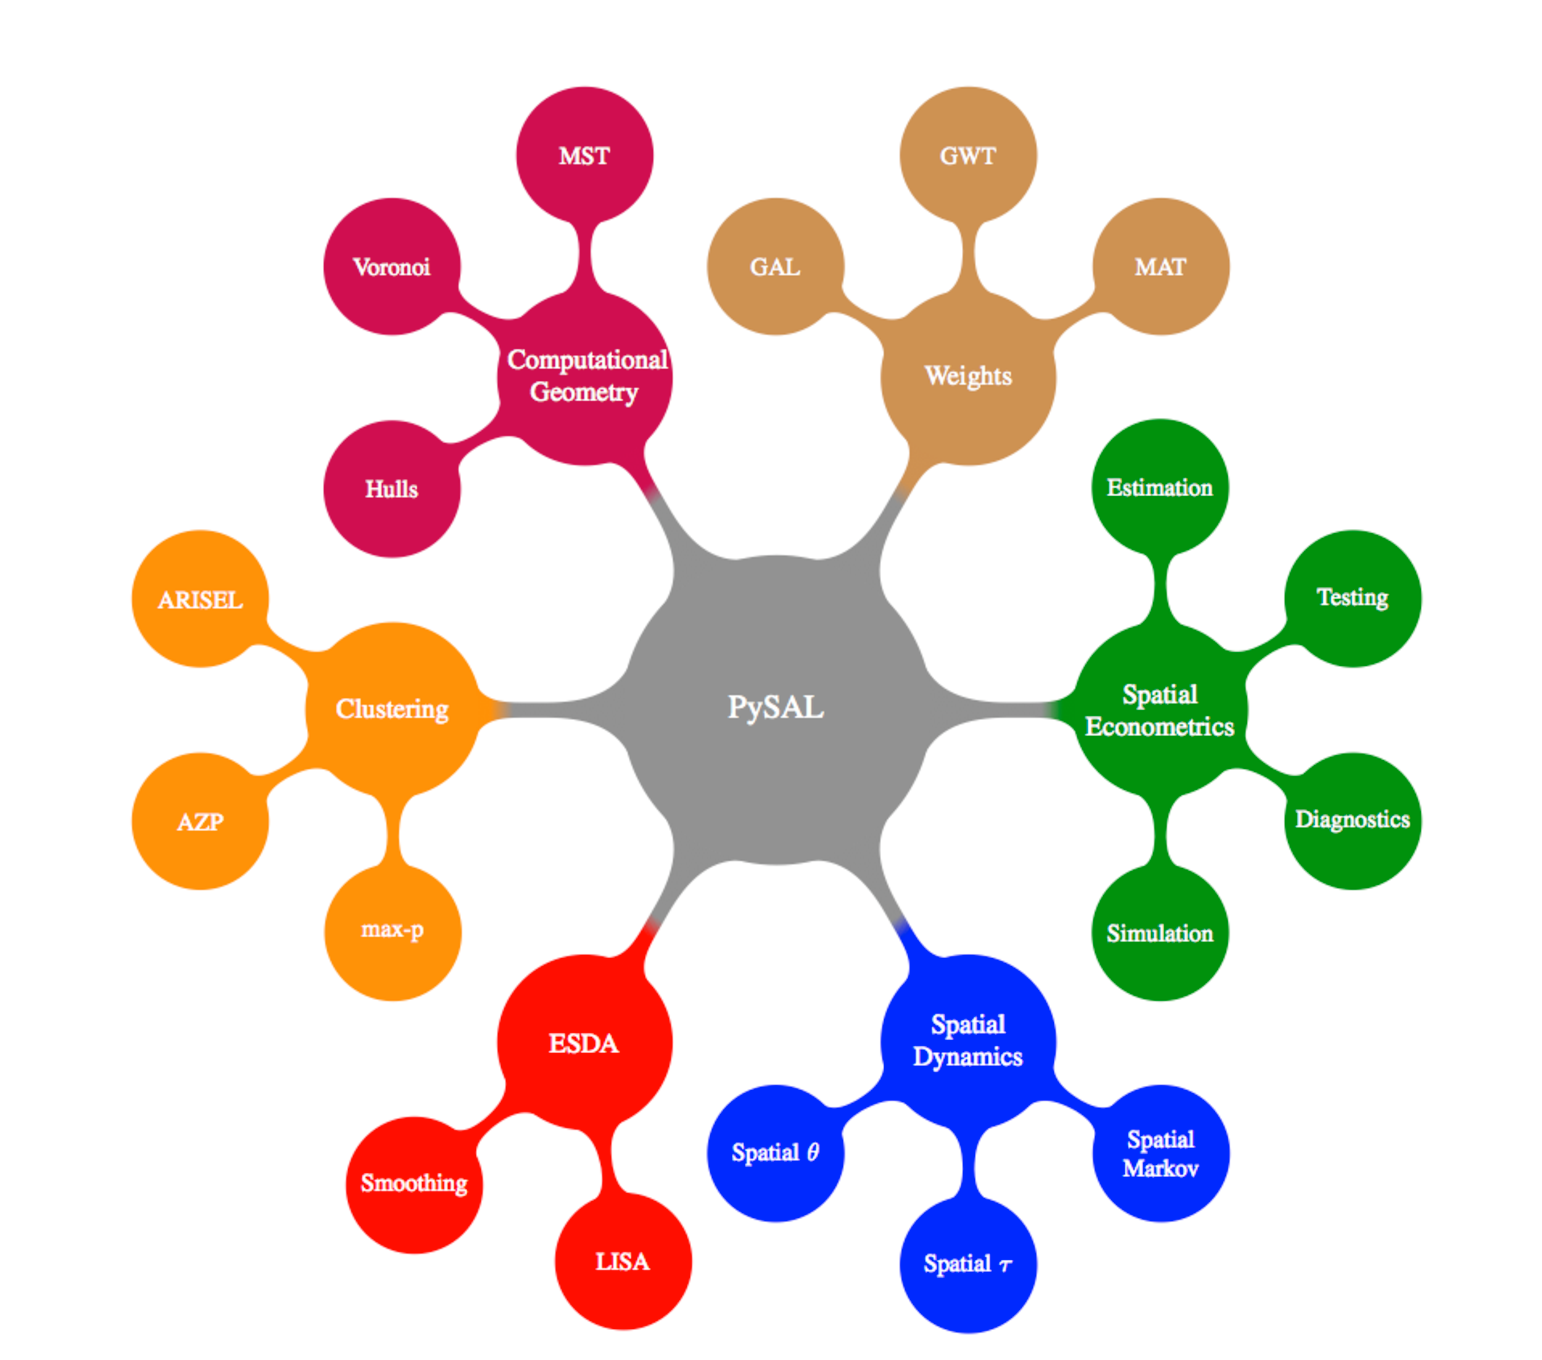
\includegraphics[width=\linewidth]{pysal_components.pdf}
\end{center}
\caption{PySAL Components}
\label{f:pysal}
\end{figure}   

\subsection{Spatial Weights}

At the core of many spatial analytical techniques is formal
representation of neighbor relations between observations embedded in
geographical space. There are a wealth of approaches to defining these
relations and the weights module implements many of the most widely
used, as well as lesser known, methods. Given their centrality in
analysis, efficiency in memory footprint and computations involving the
weights has been a high priority of our development. These efficiencies
derive from heavy use of sparse matrix methods, implemented in the
package SciPy \citep{Oliphant:2007ul}, and allow us to scale our
analytics up to large problem sizes, where large can be on the order of
several million observations in social science applications.

Interoperability has also been a guiding principle in PySAL's
development and we have placed much emphasis on supporting a wide array
of spatial weights data structures from other packages. These include
XXXX. Interoperability includes not only read support but also
conversion between these different formats and write support.

The weights module also has highly optimized methods for extracting
topology from polygon shapefiles to generate rook or queen based spatial
weight structures. The weights class itself has a number of useful
methods such as checking for asymmetries in the neighbor relations,
detection of islands (disconnected observations) and the support of
various transformations on the weights including row standardization,
double standardization and variance standardization.

\subsection{Computational Geometry}

Many of the modules in PySAL make use of computational geometry
algorithms, and we have centralized the latter in the computational
geometry module. For example, given a set of points, the CG module
supports the construction of a number of data structures including:
Voronoi tessellations and minimum spanning trees, Gabriel graphs, sphere
of influence graphs and relative neighbor graphs. These in turn can be
used by the weights module to define neighbor relations. The CG module
also implements a number of efficient spatial data indices that support
particular types of queries including point in polygon, segment
intersection, projections of points onto segments and related
operations.

\subsection{Clustering}

Methods for defining regions on a set of areal units are implemented in
the clustering module. The key approach is the max-p algorithm \citep{duque2012max}  which is
a heuristic that attempts to find the maximum number of regions that
satisfy some minimum floor constraint, such as the size of the
population in a region or the number of areas combined, while maximizing
intraregional homogeneity subject to a contiguity constraint. A key
distinguishing feature of this algorithm is the  number of regions
formed is endogenous, rather than having to be specified a-prior by the
user. Also in the clustering module are a set of methods to generate
synthetic regions that respect the cardinality of solutions from the
max-p algorithm. These provide a mechanism to evaluate the quality of
the heuristic solution.

\subsection{Exploratory Spatial Data Analysis (ESDA)}

Methods for global and local spatial autocorrelation analysis form the
core of the PySAL ESDA module. The global methods include the analysis
of binary outcomes via join count statistics with inference based on
both normal approximations as well as permutation based approaches. For
continuous variables, global version of Geary's C, Moran's I and the
Getis-Ord G statistics are included, again with multiple approaches to
inference. Local autocorrelation statistics include the local Moran and
LISA statistics, and local versions of the Getis-Ord G statistics.

In addition the these standard measures for autocorrelation analysis,
the ESDA module also includes bivariate Moran statistics as well as a
suite of approaches for continuous variables that are rates, expressed
as a ratio of the count of some event over a population at risk, where
special care is needed due to variance instability of the attribute
reflecting heterogeneity in the population at risk over the enumeration
units.

\subsection{Spatial Dynamics}

The spatial dynamics module initially was based on the space-time
analytics from STARS but has grown with the addition of a number of
newly developed methods. Three broad sets of space-time analytics are
currently implemented. The largest are Markov based methods, which
depart from the classic discrete state Markov chain (DSMC). DSMCs have
been widely used in spatial analysis to model dynamics of many spatial
processes including land use change, migration, industrial structure and
regional inequality dynamics among others. XXXget cites. PySAL extends
the DSMC in a number of directions to include a consideration of the
role of space in shaping transition dynamics. \textbf{Spatial Markov}
chains, first introduced by \cite{Rey:2001of} allow for the influence of regional
context which can introduce a form of spatial heterogeneity in the
dynamics. Later in this chapter, I will illustrate the use of these two
sets of methods.

In addition to the spatial Markov chain, the spatial dynamic module also
includes a \textbf{LISA Markov} which measures the transitions of
observations across the four quadrants of the Moran Scatter plot (from
the ESDA module) thus extending the LISA to a dynamic context. A
decomposition of the LISA Markov generates a pair of derived chains, one
for the focal unit and one for the spatial lag which in turn provide the
basis for formal tests of the independence of the transitional dynamics
for the lag and the focal chains. The combined use of the LISA Markov,
together with the focal and lag marginal chains supports the development
of a rich taxonomy of space-time dynamics as illustrated in XXXjk.

\subsection{Spatial Econometrics}

Modern methods of spatial econometrics are implemented in the spreg
module of PySAL. These include estimation methods of general method of
moments for the spatial error model, spatial lag model, combination
model as well as spatial regimes where various forms of spatial
heterogeneity are permitted across subsets of the observations.

In addition to state of the art estimation methods, spreg includes an
array of spatial and non-spatial diagnostics and handles non-spatial
endogenous variables. The spreg module supports the use of a rich set of
spatial weights including various contiguity criteria, distance bands,
knn neighbors and inverse distance as well as kernel based weights
required by the heteroskedasticity and autocorrelation consistent (HAC)
estimators.

XXX flesh out

\section{PySAL Use cases}

By design PySAL as a library is intended to support a variety of
delivery mechanisms and use cases. This is a recognition of the
diversity of end users and computing platforms that spatial analytical
services are consumed on. Figure~\ref{f:use} gives an overview of the
possible relationships between PySAL and other platforms.

\begin{figure}[ht]
\begin{center}
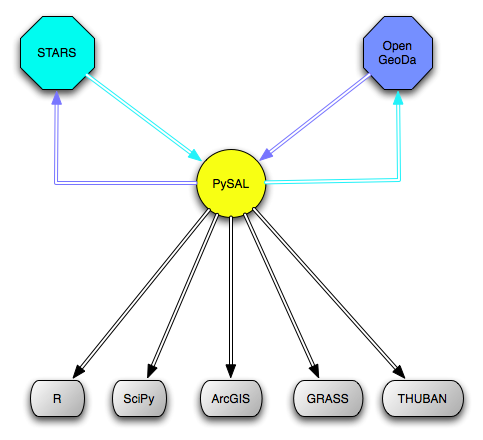
\includegraphics[width=\linewidth]{pysal_applications.png}
\end{center}
\caption{PySAL Use Cases}
\label{f:use}
\end{figure}   


\paragraph{Interactive computing}

In many areas of scientific investigation, often one does not have a
clear hypothesis in mind and instead adopts an exploratory, or data
driven, approach to the analysis. Here the use of an interactive prompt
is invaluable as the ultimate scientific work-flow is not readily
apparent, and instead, the next computational task that the research
will apply is only known after the results of the previous step are
generated. PySAL supports interactive computing using either the built
in Python interpretor or the more powerful IPython Notebook. This latter
will be illustrated in the empirical example below.

\paragraph{Graphical User Interface Clients}

A second use case the PySAL supports is the wrapping of components of
the library in rich desktop clients which provide access to the
underlying functionality through a user-friendly graphical user
interface (GUI). One such example is the package Crime Analytics for
Space-Time (CAST). Figure \ref{f:cast} shows one selected CAST window
which is illustrative of the kind of functionality it supports. CAST
enables the joint consideration of multiple types of spatial supports
(polygon, point, network) in a powerful and flexible set of fully
interactive dynamic graphics. Also shown are calendar maps that provide
insights as to the temporal distribution of crime events.

\begin{figure}[ht]
  \begin{center}
    \includegraphics[width=\linewidth]{src/cast.png}
  \end{center}
     \caption{CAST: Crime Analytics for Space-Time}
     \label{f:cast}
      \end{figure}      

The specialized nature of CAST is emblematic of a development philosophy
at the Center where end user applications are tightly focused on the
spatial analytical functionality most appropriate to a substantive
problem domain. Rather than attempting to develop a one-size fits all
GUI based application, the wide scope of methods in the PySAL engine can
be selected from to develop tailored applications in a time efficient
manner.

Another prominent example of a stand-alone application built around a
PySAL core is the package GeoDaSpace. XXX

\paragraph{GIS Toolkits}

In addition to interactive shells and GUI clients, users can interface
with PySAL through toolkit architectures of geographic information
systems (GIS) such as ArcGIS and QGIS. Figure \ref{f:arcgis} displays an example of an
early version of a toolbox for ArcGIS 10.1.\footnote{At the time of
  writing the ArcGIS toolbox is in Alpha with a stable release planned
  for spring 2014.}

%\begin{figure}[ht]
%  \begin{center}
%    \includegraphics[width=\linewidth]{src/10_arctool.png}
%  \end{center}
%     \caption{ArcGIS PySAL Toolbox}
%     \label{f:arcgis}
%      \end{figure}      

\begin{figure}[ht]
\begin{center}
\includegraphics[width=\linewidth]{src/10_arctool.png}
\end{center}
\caption{ArcGIS PySAL Toolbox}
\label{f:arcgis}
\end{figure}   


\paragraph{Web Services}

A final delivery mechanism for PySAL is through web services. These make
a selection of the spatial analytic functionality available to the end
user via a browser. An example can be seen in Figure~\ref{f:cgpysal}
which shows the interface to spreg on the CyberGIS Gateway \citep{Wang:2010sg}.
Here the user can upload their own data and then, using a flexible drag
and drop interface select variables to
specify a model. Once the model is defined alternative options can be
specified (as shown). 

\begin{figure}[ht]
\begin{center}
\includegraphics[width=\linewidth]{src/cgpysal}
\end{center}
\caption{PySAL Spatial Regression in the CyberGIS Gateway}
\label{f:cgpysal}
\end{figure}   

In addition to enabling distributed computing whereby endusers no longer
require local installation of software, the centralized installation of
PySAL as part of the CyberGIS Gateway allows us to implement a highly
optimized version of PySAL that fully exploits the characteristic of the
underlying hardware. This results in computational gains that are
generally not available in the version of PySAL that is available for
users to install locally since we focus on general portability in that
version rather than targeting specific hardware. 


\section{Illustration}

Given the scope of the modules in PySAL space limitations prevent an
exhaustive set of illustrations. Instead I focus on one particular
module, spatial dynamics, and a case study exploring the dynamics of
homicide patterns in  1,412 southern US counties using data developed as part of an
broader project \citep{Baller:2001aa, Messner:1999xz}.

XXX flesh out substantive issues

diffusion
contagion
violence
comparative statics
motivate focus on the south

\subsection{Spatial Distribution of Homicide Rates}

Figure~\ref{f:hr} shows choropleth maps for the homicide rates
(HR=homicides per 100,000) using a quintile classification for the
decades of 1960-1990. The classification method is one of the options in
the PySAL map classification module and it is used here with the
visualization module which is a contributed module. The latter are user
inspired modules that are not formally part of the core PySAL library
but provide a way for users to extend the library for particular use
cases.


\begin{figure}
  \centering
  \subfloat[1960]{\includegraphics[width=.5\linewidth]{src/quantiles_HR60.png}}
  \subfloat[1970]{\includegraphics[width=.5\linewidth]{src/quantiles_HR70.png}}
  \\
  \noindent
  \subfloat[1980]{\includegraphics[width=.5\linewidth]{src/quantiles_HR80.png}}
  \subfloat[1990]{\includegraphics[width=.5\linewidth]{src/quantiles_HR90.png}}
\caption[caption]{Homicide Rates 1960-90}
\label{f:hr}
\end{figure}


Examination of the class boundaries indicates that the lower four
quintiles are fairly stable over the four decades, while the maximum
value is highest in the first decade (92.94), drops in the intermediate two
decades and then rises up to 64.26 in 1990. An a-spatial view of the
distribution dynamics is portrayed in Figure~\ref{f:bp} suggests that the overall level
of homicide was actually lower in the first and last decade, relative to
the middle two decades if the medians are considered.


\begin{figure}[ht]
\begin{center}
\includegraphics[width=\linewidth]{src/bp.png}
\end{center}
\caption{Box Plots Homicide Rate 1960-1990}
\label{f:bp}
\end{figure}   


Applying Moran's $I$ to the homicide rates for each decade reveals
significant positive spatial autocorrelation and these measures are
robust to choice of the spatial weights matrix (rook versus queen) in
all periods.

Table with I EI psim.

\subsection{Spatial Distributional Dynamics}

The global measures of autocorrelation are similar over this period
suggesting that the pattern of homicide activity may be relatively
stable. Similarly, the stability of the majority of the quintiles may
also be interpreted as evidence of distributional stability. However,
both sets of measures are global, or whole map, measures that may mask
more complex dynamics at work \emph{within} the distribution. PySAL's
spatial dynamic module has a number of space-time analytics that
consider the role of space in the evolution of distributions over time.

\subsubsection{Discrete Markov Chains}

The first of these is based on a classic discrete Markov chain which
uses the quintiles to define the states of the chain. More specifically,
the homicide rate in each county is viewed as a sample chain that can
take one of five discrete values corresponding to its position in the
quintile distribution in a given year. By pooling all the sample chains,
the probability transition matrix can be estimated via maximum
likelihood as:

\begin{equation}
\hat{p}_{i,j} = \frac{\sum_t n_{i,j,t}}{\sum_t \sum_j n_{i,j,t}} 
\label{e:cm}
\end{equation}
where $n_{i,j,t}$ is the number of times a sample chain started in state $i$
in period $t$ and transitioned to state $j$ in the next period. Applying this estimator
to our sample chains gives the  estimated transition
probability matrix $P$ in Table \ref{t:cm}

\begin{table}
  \centering
  \small
\begin{tabular}{|l|lllll|}\hline
   &  &  &t+10& & \\
  t&Q1&Q2&Q3&Q4&Q5\\
  \hline
   Q1& 0.431&0.253&0.128&0.099&0.088\\
   Q2& 0.240&0.291&0.241&0.145&0.083\\
   Q3& 0.154&0.214&0.277&0.221&0.135\\
   Q4& 0.106&0.150&0.215&0.271&0.258\\
   Q5& 0.071&0.091&0.138&0.263&0.438\\
    \hline
    $\pi$&0.200&0.200&0.200&0.200&0.200\\
    \hline
\end{tabular}
\caption{Homicide rate transition probabilities}
\label{t:cm}
\end{table}

There is strong evidence of mobility in the homicide rate distribution
as the probability of remaining in the same quintile over sequential
decades is less than 0.50 for all quintiles. The mobility is higher for
the intermediate quintiles than is the case for the first and last
quintiles. Lower mobility for the fifth class is to be expected given
the skewed nature of the homicide rate distribution in each decade which
results in a wider interval for that state in the Markov chain. Interval
width alone, however, does not account for the lower mobility in the
first quintile as its width is similar to that of the fourth quintile.

The last row in Table~\ref{t:cm} is the estimated long run steady state
distribution $\pi$ which suggests a uniform distribution holds when the chain
reaches equilibrium. Note that although the states of the chain are
defined using the quintiles of the distribution, this does not imply
that the ergodic distribution will necessarily be uniform. In other
words, there is no evidence of a convergence of homicide rates into
particular parts of the distribution in the long run.

\subsubsection{Spatial Markov Chains}

The classic discrete Markov chain provides a first view of the
distributional dynamics, however, it does not consider the spatial
location of the sample chains and how the local context of a county
might effect the chain's movement in the distribution and transitions
across states. One approach to consider this is the spatial Markov chain
which conditions the transition dynamics of a county's homicide rate on
the spatial lag of homicide rates. In other words rather than a single
transition probability matrix $P$, counties may face a different
transition matrix depending on their spatial context.

Use of the spatial Markov class in PySAL estimates the conditional
transition probability matrices reported in Table \ref{t:sm}. The matrices are
ordered according to the value of a chain's spatial lag at the beginning
of the transition period, so that the first conditional matrix $P(1)$ is
for chains who had neighbors with homicide rates in the lowest quintile,
and the last matrix $P(5)$ is for chains with spatially lagged homicide
rates falling in the upper quintile. These are estimated using:

\begin{equation}
\hat{p}(l)_{i,j} = \frac{\sum_t n(l)_{i,j,t}}{\sum_t \sum_j n(l)_{i,j,t}} 
\label{e:cm}
\end{equation}
where $n(l)_{i,j,t}$ is the number of times a sample chain with a
spatial lag in quintile $l$ started in state $i$
in period $t$ and transitioned to state $j$ in the next period.

Examination of the table reveals that the spatial context of a chain can
influence its transition dynamics over a decade. Counties that have
homicide rates in the fifth quintile face different probabilities of
remaining in that quintile depending on whether their surrounding
counties also have rates in the upper quintile ($p(5)_{5,5} = 0.383$),
or if the neighbors fall in the fourth quintile ($p(4)_{5,5}=0.462$). At
the other end of the spectrum, counties with the lowest homicide rates
face a higher propbability of remaining in the first quintile when their
neighbors are also in the first quintile ($p(1)_{1,1}=0.528$) relative
to when the neighbors' rate falls in the second quintile
($p(2)_{1,1}=0.473$). A formal test for the heterogeneity of the
transition probabilities across lag quintiles rejects the null (H\_o:
$P=P(l) \ \forall l=\{1,2,\ldots,k\})$of a single homogeneous transition
probability matrix $\chi_{(80)}^2=454.27, p<0.001$.

\begin{table}
  \centering
  \small
\begin{tabular}{|ll|lllll|}\hline
    & & & & t+10& & \\
    & t& Q1& Q2& Q3& Q4& Q5\\
    \hline
    & Q1&  0.528& 0.218& 0.106& 0.095& 0.053\\
    & Q2&  0.382& 0.259& 0.195& 0.109& 0.055\\
P(1)& Q3&  0.271& 0.243& 0.250& 0.194& 0.042\\
    & Q4&  0.288& 0.192& 0.219& 0.137& 0.164\\
    & Q5&  0.352& 0.074& 0.259& 0.111& 0.204\\
    \hline
    & $\pi(1)$& 0.408& 0.217& 0.176& 0.122& 0.076\\
    \hline
    & Q1& 0.473& 0.268& 0.123& 0.077& 0.059\\
    & Q2& 0.219& 0.321& 0.232& 0.161& 0.067\\
P(2)& Q3& 0.235& 0.246& 0.278& 0.182& 0.059\\
    & Q4& 0.218& 0.155& 0.211& 0.261& 0.155\\
    & Q5& 0.096& 0.233& 0.192& 0.178& 0.301\\
    \hline
    & $\pi(2)$& 0.281& 0.256& 0.203& 0.159& 0.101\\
    \hline
    & Q1& 0.299& 0.328& 0.164& 0.104& 0.104\\
    & Q2& 0.218& 0.326& 0.249& 0.130& 0.078\\
P(3)& Q3& 0.076& 0.240& 0.292& 0.263& 0.129\\
    & Q4& 0.091& 0.217& 0.202& 0.293& 0.197\\
    & Q5& 0.053& 0.127& 0.167& 0.273& 0.380\\
    \hline
    & $\pi(3)$& 0.142& 0.250& 0.222& 0.215& 0.170\\
    \hline
    & Q1& 0.210& 0.309& 0.173& 0.123& 0.185\\
    & Q2& 0.143& 0.286& 0.316& 0.150& 0.105\\
P(4)& Q3& 0.119& 0.206& 0.299& 0.216& 0.160\\
    & Q4& 0.045& 0.104& 0.270& 0.284& 0.297\\
    & Q5& 0.042& 0.083& 0.125& 0.287& 0.463\\
    \hline
   & $\pi(4)$&  0.094& 0.173& 0.237& 0.230& 0.265\\
    \hline
    & Q1& 0.286& 0.161& 0.143& 0.161& 0.250\\
    & Q2& 0.118& 0.211& 0.250& 0.237& 0.184\\
P(5)& Q3& 0.073& 0.127& 0.253& 0.253& 0.293\\
    & Q4& 0.047& 0.118& 0.171& 0.289& 0.374\\
    & Q5& 0.048& 0.053& 0.104& 0.284& 0.511\\
    \hline
    & $\pi(5)$& 0.078& 0.108& 0.165& 0.265& 0.383\\
    \hline
\end{tabular}
\caption{Spatially conditioned transition probability matrices}
\label{t:sm}
\end{table}

The spatial heterogeneity in the transition probabilities also has
implications for the estimated long run distribution of homicide rates.
Recall that under the assumption homogeneity (\ref{e:cm}), the long run
distribution is uniform across the five classes. By contrast, there are
five separate estimated conditional ergodic distributions in Table
\ref{t:sm},
none of which are uniform. The mass of the distribution moves towards
the tail of the distribution reflected in the value of the conditional
lag - for example, the distribution conditioned on the first lag
quintile is right skewed, while the distribution conditioned on the
fifth lag quintile is left skewed. Moreover, the long run distribution
conditioned on the central lag departs from uniformity as the mass moves
out of both tails and into the central three classes.


\subsubsection{LISA Markov}
The spatial Markov provides insight as to the role of regional context
at the beginning of a transition period in influencing the movement of a
county's homicide rate within the distribution over time. In other
words, different spatial contexts can give rise to different dynamics.
Those conditional dynamics, however, give rise to new realizations of
the spatial lag for each county in the next period, and the question of
how the county's homicide rate may co-evolve with its spatial lag
naturally arises.

The spatial dynamic modules includes several analytics designed to
address this question. One way to visualize the co-movement of a
county's homicide rate with that of its spatial lag is to consider the
origin standardized movement vector obtained from comparing Moran
Scatter Plots \citep{Anselin:1996ze} from sequential decades.
Figure~\ref{f:lmplot} pools all the movement vectors over the three
transitions (1960-70, 1970-80, 1980-80) which  provides an impression of
the directional tendencies in the distributional dynamics. One striking
feature is the relative asymmetry of the lengths of the movement vectors
when considering the focal unit dimension (x-axis) versus the spatial lag
dimension (y-axis). This is to the spatial lag operator being a weighted
average of homicide rates, whereas the for the focal unit only the raw
rate is considered. Thus the latter will tend to have variances that are
greater than or equal to those of the lag.


It is important to note that the movement vectors reflect
\emph{relative} movement of a LISA within two scatter plots, and not
\emph{absolute} movements.  In other words movements to the southwest in
Figure~\ref{f:lmplot} indicate a county's homicide rate was declining in
concert with a decline in value for its spatial lag. Similarly,
movements to the northeast represent increases in the focal county's
homicide rate and that found in its neighboring counties between two
periods. These do not necessarily represents movements between quadrants
in the Moran Scatter Plot.


\begin{figure}[ht]
\begin{center}
\includegraphics[width=\linewidth]{src/lmplot.png}
\end{center}
\caption{Origin standardized LISA movement vectors for homicide rates}
\label{f:lmplot}
\end{figure}   

If we slightly abuse the notion of an ``absolute move'' to define it as a
movement across one of the four quadrants of the Moran Scatter plot, we
can define a LISA Markov  where the states of the chain
are taken as the four quadrants of a Moran Scatter Plot in a given
period: (HH=1, LH=2, LL=3, HL=4) where HL indicates that the crime rate
in the county was above the average for that period while its spatial
was below average.  Between any two decades a county's position in the
Moran Scatter Plot may change to transition between the quadrants.
Collecting all these transitions allows for the estimation of a LISA
Markov transition probabilities reported in Table~\ref{t:lm}. 

Examination of these probabilities reveals several
interesting characteristics about the spatial dynamics of homicide rates.
First, the staying probabilities (i.e., probability of remaining in one
state of the space) are highest for quadrants 1 and 3 of the scatter
plot. This is indicative of relative stability in positive spatial
autocorrelation that we encountered in the application of the global
Moran's I statistic earlier. Second, the estimated equilibrium
distribution for the LISA chain is to have the mass of the distribution
more concentrated in these two classes (amounting for almost two-thirds
of the distribution), again reflecting the dominant pattern of spatial
clustering.

\begin{table}
  \centering
  \small
\begin{tabular}{|l|llll|}\hline
  & &t+10 & &\\
  t&HH&LH&LL&HL\\
  \hline
HH&0.615 &0.210 &0.083 &0.093\\
LH&0.327 &0.336 &0.246 &0.091\\
LL&0.063 &0.107 &0.675 &0.156\\
HL&0.190 &0.124 &0.411 &0.275\\
\hline
$\pi$&0.287 &0.180 &0.390 &0.143\\
\hline
\end{tabular}
\caption{LISA Markov transition probabilities}
\label{t:lm}
\end{table}

A third pattern seen in Table~\ref{t:lm} is that when movements out of a
quadrant do occur they are more likely to reflect the contribution of
the movement of the homicide rate in the focal county than they are the
movement of the spatial lag. For example, considering the chains in the
initial state HH, the movement to LH which involves an absolute change
for the focal unit rate but not the spatial lag, occurs more frequently
than movement to HL which involves a change in the absolute position of
the lag but not the focal rate. Similarly for an initial state of LL,
moves to HL are more frequent than moves to LH. These patterns reflect
the asymmetry in the magnitudes of the movement vectors in
Figure~\ref{f:lmplot} alluded to previously.


Joint chain


\begin{table}
  \centering
  \small
\begin{tabular}{|rrrr|}\hline
756 &258 &102 &114\\
244 &251 &184 &68\\
103 &175 &1105 &255\\
118 &77  &255 &171\\
\hline
338 &310 &278 &303\\
173 &221 &198 &155\\
357 &457 &463 &361\\
161 &148 &150 &163\\
\hline
\end{tabular}
\caption{Observed versus expected joint spatial chain transitions}
\label{t:jc}
\end{table}



\subsubsection{Summary}
The spatial dynamics module applied to the case of homicide data has
revealed clear evidence of spatial contextual effects in shaping the
evolution of homicide activity distributions over space and time. At the
same time it is important to keep in mind that the patterns identified
are indirect evidence of spatial diffusion processes and do not imply a
particular causal structure. The latter requires confirmatory modeling
that reflects specific structural mechanisms giving rise to the patterns
identified here. Nevertheless, detection of the patterns via the
application of exploratory space-time methods suggests that such investigation is
warranted.

\section{Conclusion}

One of the strengths of open source spatial analysis projects is that
through the efforts of development teams, new state of the art methods
appearing in the scientific literature are often implemented in
libraries that serve an important dissemination function. In this
regard, PySAL shares in this effort, yet, a unique unique feature of the
PySAL project is that several of the core developers have also been the
creators of new spatial analytical methods that then become components
of the library. By building on the contributions of others, this has
allowed us to focus on the parts of the spatial analytical research
stack where our expertise can have the most impact.

Cite other empirical studies making use of PySAL or reporting on methods
development. XXX

Our targeting of the Python language and scientific community is
sometimes questioned by spatial scientists who are more familiar with R
and the ecosystem of associate spatial packages, as the implication is
that we are diverting energies that should otherwise be directed towards
R. While we understand the sentiment behind such questions, we think
they are somewhat misplaced for several reasons. First, at the time of
PySAL's conception, Python was beginning to make major inroads into
scientific computing, yet spatial analysis was largely absent. We felt
that focusing on Python would serve an important dissemination mechanism
whereby leading developments in spatial analysis could be brought to new
communities. The inclusion of PySAL in Anaconda is evidence that we have
achieved some success in this regard. Secondly, we do not see our
efforts as duplicative of the excellent work in the R related projects.
Moreover, with new tools like the IPython notebook, it is now possible
to use R and PySAL together in the same workflow. From this perspective,
developments in either project R or PySAL can serve to benefit the
other.

PySAL is well situated to contribute to an evolving CyberGIS
infrastructure, and several ongoing projects are focused on embedding
PySAL in HPC environments. The notion of spatial analytical work-flows
requires frameworks for trackign the provenance of a sequence of
analytical operations that are chained together to produce a result. We
are currently exploring a prototype of such a provenance framework that
captures the work flow in a distributed context and would support full
replication of results.

Closely related to this work is the development of a spatial
econometrics workbench \citep{Anselin:2011wt} that would target spatial econometrics in
particular but bring the methods from the spreg module of PySAL into a
distributed available to reseachers to access through web browsers .

provenance and meta data

play an important role in an evolving CyberGIS infrastructure

\bibliographystyle{apa}
%\bibliography{/Users/serge/Dropbox/bib/library}
\bibliography{/Users/serge/Dropbox/bib/library}
\end{document}
